\subsection{Template Page}

A template in a web application refers to a pre-designed layout or structure that can be customized to create a new web page or website.\\

Templates typically include the basic elements of a web page, such as headers, footers, navigation menus, and content sections, which can be modified to fit the specific needs of the user.\\

Templates can be created from scratch, or they can be downloaded from a library of pre-built templates, which are often available for free or for a fee.\\

Web developers and designers use templates to save time and streamline the web development process.
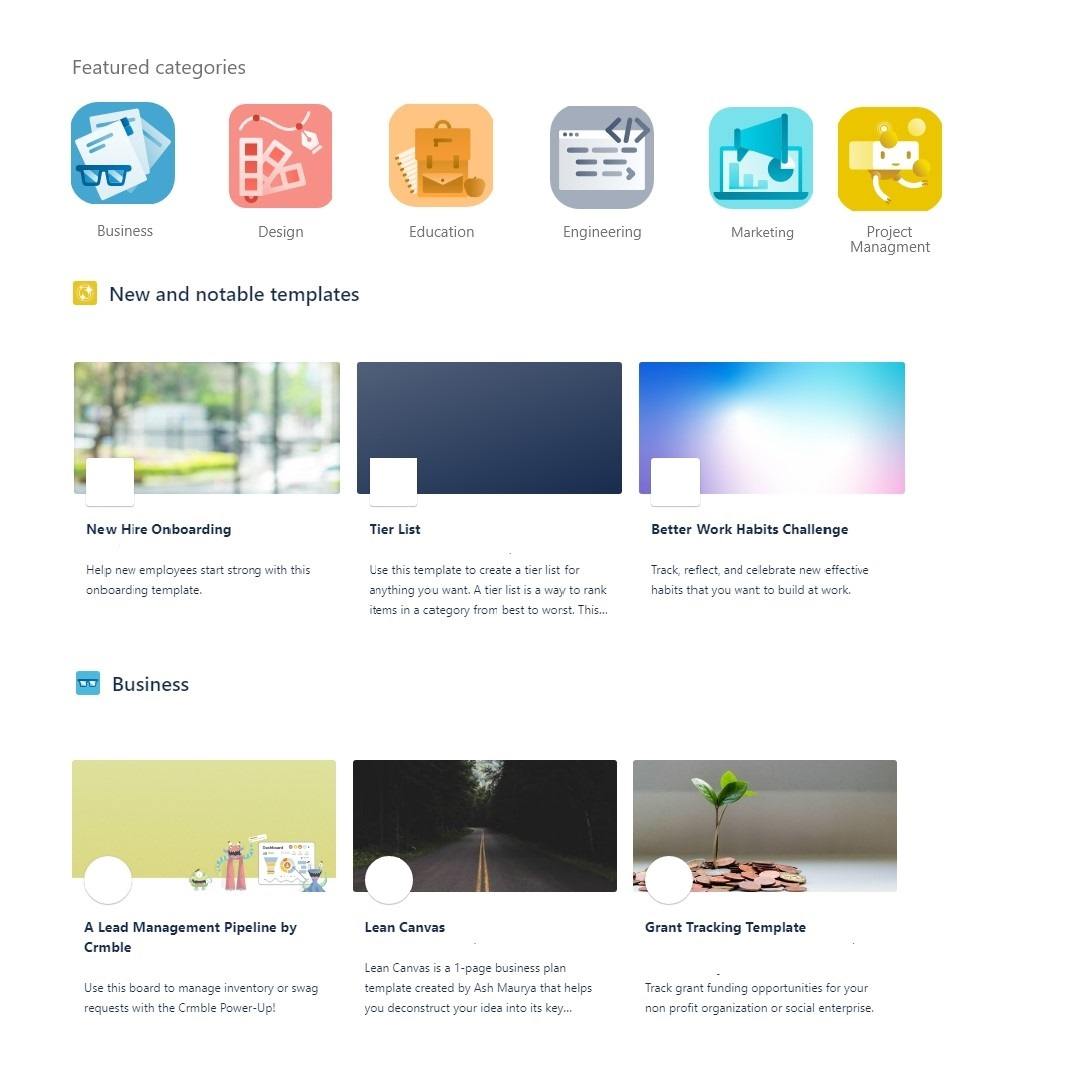
\includegraphics[width=0.8\columnwidth]{images/template.jpg}
